\section{Exercícios}

\begin{exercise}
Descubra os valores de $x$ de modo que seja possível completar
o preenchimento do quadrado mágico abaixo:
\begin{center}
\begin{tabular}{|c|c|c|}
  \hline
   \ \ \  & \ \ \  & \ \ \  \\ \hline
          & $x$    &        \\ \hline
          &        &        \\
  \hline
\end{tabular}
\end{center}
\end{exercise}

\begin{exercise}
Observe as multiplicações a seguir:
\begin{enumerate}[i.]
  \item $12.345.679 \cdot 18 = 222.222.222$
  \item $12.345.679 \cdot 27 = 333.333.333$
  \item $12.345.679 \cdot 54 = 666.666.666$
\end{enumerate}
Para obter 999.999.999 devemos multiplicar 12.345.679 por quanto?
\end{exercise}

\begin{exercise}
Com algarismos $x$, $y$ e $z$ não todos nulos formam-se os
números de dois algarismos $xy$ e $yx$, cuja soma é o número de três
algarismos $zxz$. Quanto valem $x$, $y$ e $z$?
\end{exercise}

\begin{exercise}
Quantos são os números inteiros de 2 algarismos que são iguais
ao dobro do produto de seus algarismos?
\end{exercise}


\begin{exercise}
O número $-3$ é a raiz da equação $x^2 -7x -2c = 0$. Nessas
condições, determine o valor do coeficiente $c$.
\end{exercise}

\begin{exercise}
  Sejam $\alpha_1$ e $\alpha_2$ as raízes da equação do 2° grau $ax^2+bx+c=0$. Calcule
  as seguintes expressões em função de $a$, $b$ e $c$:
  \begin{enumerate}[a)]
    \item \[\frac{\alpha_1+\alpha_2}{2}\]
    \item \[\sqrt{\alpha_1\cdot\alpha_2}\]
    \item \label{item:raizes-segundo-grau-ultimo} \[\sqrt{\alpha_1}+\sqrt{\alpha_2}\]
  \end{enumerate}
  \textit{Dica}: no item~\ref{item:raizes-segundo-grau-ultimo}, inicie calculando o 
  quadrado da expressão.
\end{exercise}

\begin{exercise}
Dada as frações $$\frac{966666555557}{966666555558} \; \text{ e
} \; \frac{966666555558}{966666555559},$$ qual é a maior?
\end{exercise}


\begin{exercise}
Nove cópias de certas notas custam menos de R\$ 10,00 e dez
cópias das mesmas notas (custando o mesmo preço cada uma) custam
mais de R\$ 11,00. Quanto custa uma cópia das notas? 
\end{exercise}

\begin{exercise}
Ache os valores de $x$ para os quais cada uma das seguintes
inequações é válida:
\begin{enumerate}[a)]
  \item $\dfrac x {x^2+9} > 0$;
  \item $\dfrac{x-3}{x+1} > 0$;
  \item $\dfrac{x^2-1}{x^2-3} > 0$;
  \item $\dfrac{x^2+x-6}{x^2+6x+5} \leq 0$.
\end{enumerate}
\end{exercise}

\begin{exercise}
Sejam  $a$, $b$, $c$, $d > 0$ tais que $\frac a b < \frac c d$.
Mostre que $$\frac a b < \frac {a+c} {b+d} < \frac c d.$$
\end{exercise}

\begin{exercise}
  Mostre que se $r$ e $s$ são números racionais positivos satisfazendo $r < s$,
  então existe um outro número racional $q$ tal que $r<q<s$.
\end{exercise}

\begin{exercise}
Determine o conjunto solução de cada uma das equações ou
inequações modulares abaixo:
\begin{enumerate}[a)]
  \item $\modu {3x - 5}= 7;$
  \item $\modu {-x +8} = -1;$
  \item $\modu{x^2 - 1}= 3;$
  \item $\modu{x +1} + \modu { -3x +2} = 6;$
  \item $\modu{x-1} \cdot \modu{x+2} = 3;$
  \item $\modu{x^2-1}\le 3$;
  \item $\modu{x-1}+ \modu{x+1}>2;$
  \item $\modu{x+1}- \modu{x-1}<-2.$
\end{enumerate}
\end{exercise}

\begin{exercise}
Prove que $\modu{x\cdot y } = \modu x \cdot \modu y$ para todo
$x, y \in \R$.
\end{exercise}

\begin{exercise}
Seja $x \in \R$. Mostre que:
\begin{enumerate}[a)]
    \item $\modu{x-5}<0{,}1 \implies \modu{2x - 10}< 0{,}2;$
    \item $\modu{x+3}<0{,}1 \implies \modu{-\frac 3 2 x + 3 -
    7{,}5}<0{,}15;$
    \item $\modu{x-2}< \sqrt{5} - 2 \implies \modu{x^2 - 4}< 1;$
    \item $\modu{ x - 3 } < \raiz{46} - 5 \implies \modu{ x^2 + 4x - 21 } < 21.$
\end{enumerate}
\end{exercise}


\begin{exercise}
	Quatro cidades rurais \emph{Abaeté}, \emph{Bertioga}, \emph{Caicó} e \emph{Diamantina} estão situadas geograficamente como a imagem abaixo.
	\begin{figure}[H]
		\centering
		\label{fig:exercicio-cidades}
		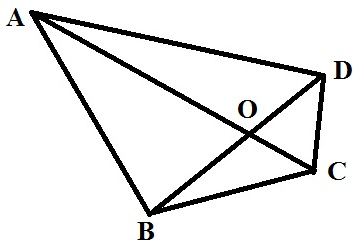
\includegraphics[scale=0.75]{\imgdirfromsection/exercicio-cidades.jpg}
		\caption{Disposição das cidades.}
	\end{figure}
	A empresa \emph{Ozymandias} deseja construir uma central de distribuição de energia para as quatro cidades de modo que a soma total das distâncias da central a cada uma das quatro cidades seja a mínima possível. Mostre que a central deve ser construída no ponto $O$, que é o ponto em comum dos segmentos $AC$ e $BD$.
\end{exercise}

\begin{exercise}
  Três círculos que não se intersectam tem seus centros colineares (sobre uma mesma reta). Um quarto círculo os tangencia, conforme a imagem abaixo. Mostre que o raio do quarto círculo é maior que pelo menos um dos outros raios.
  \begin{figure}[H]
		\centering
		\label{fig:exercicio-4circulos}
    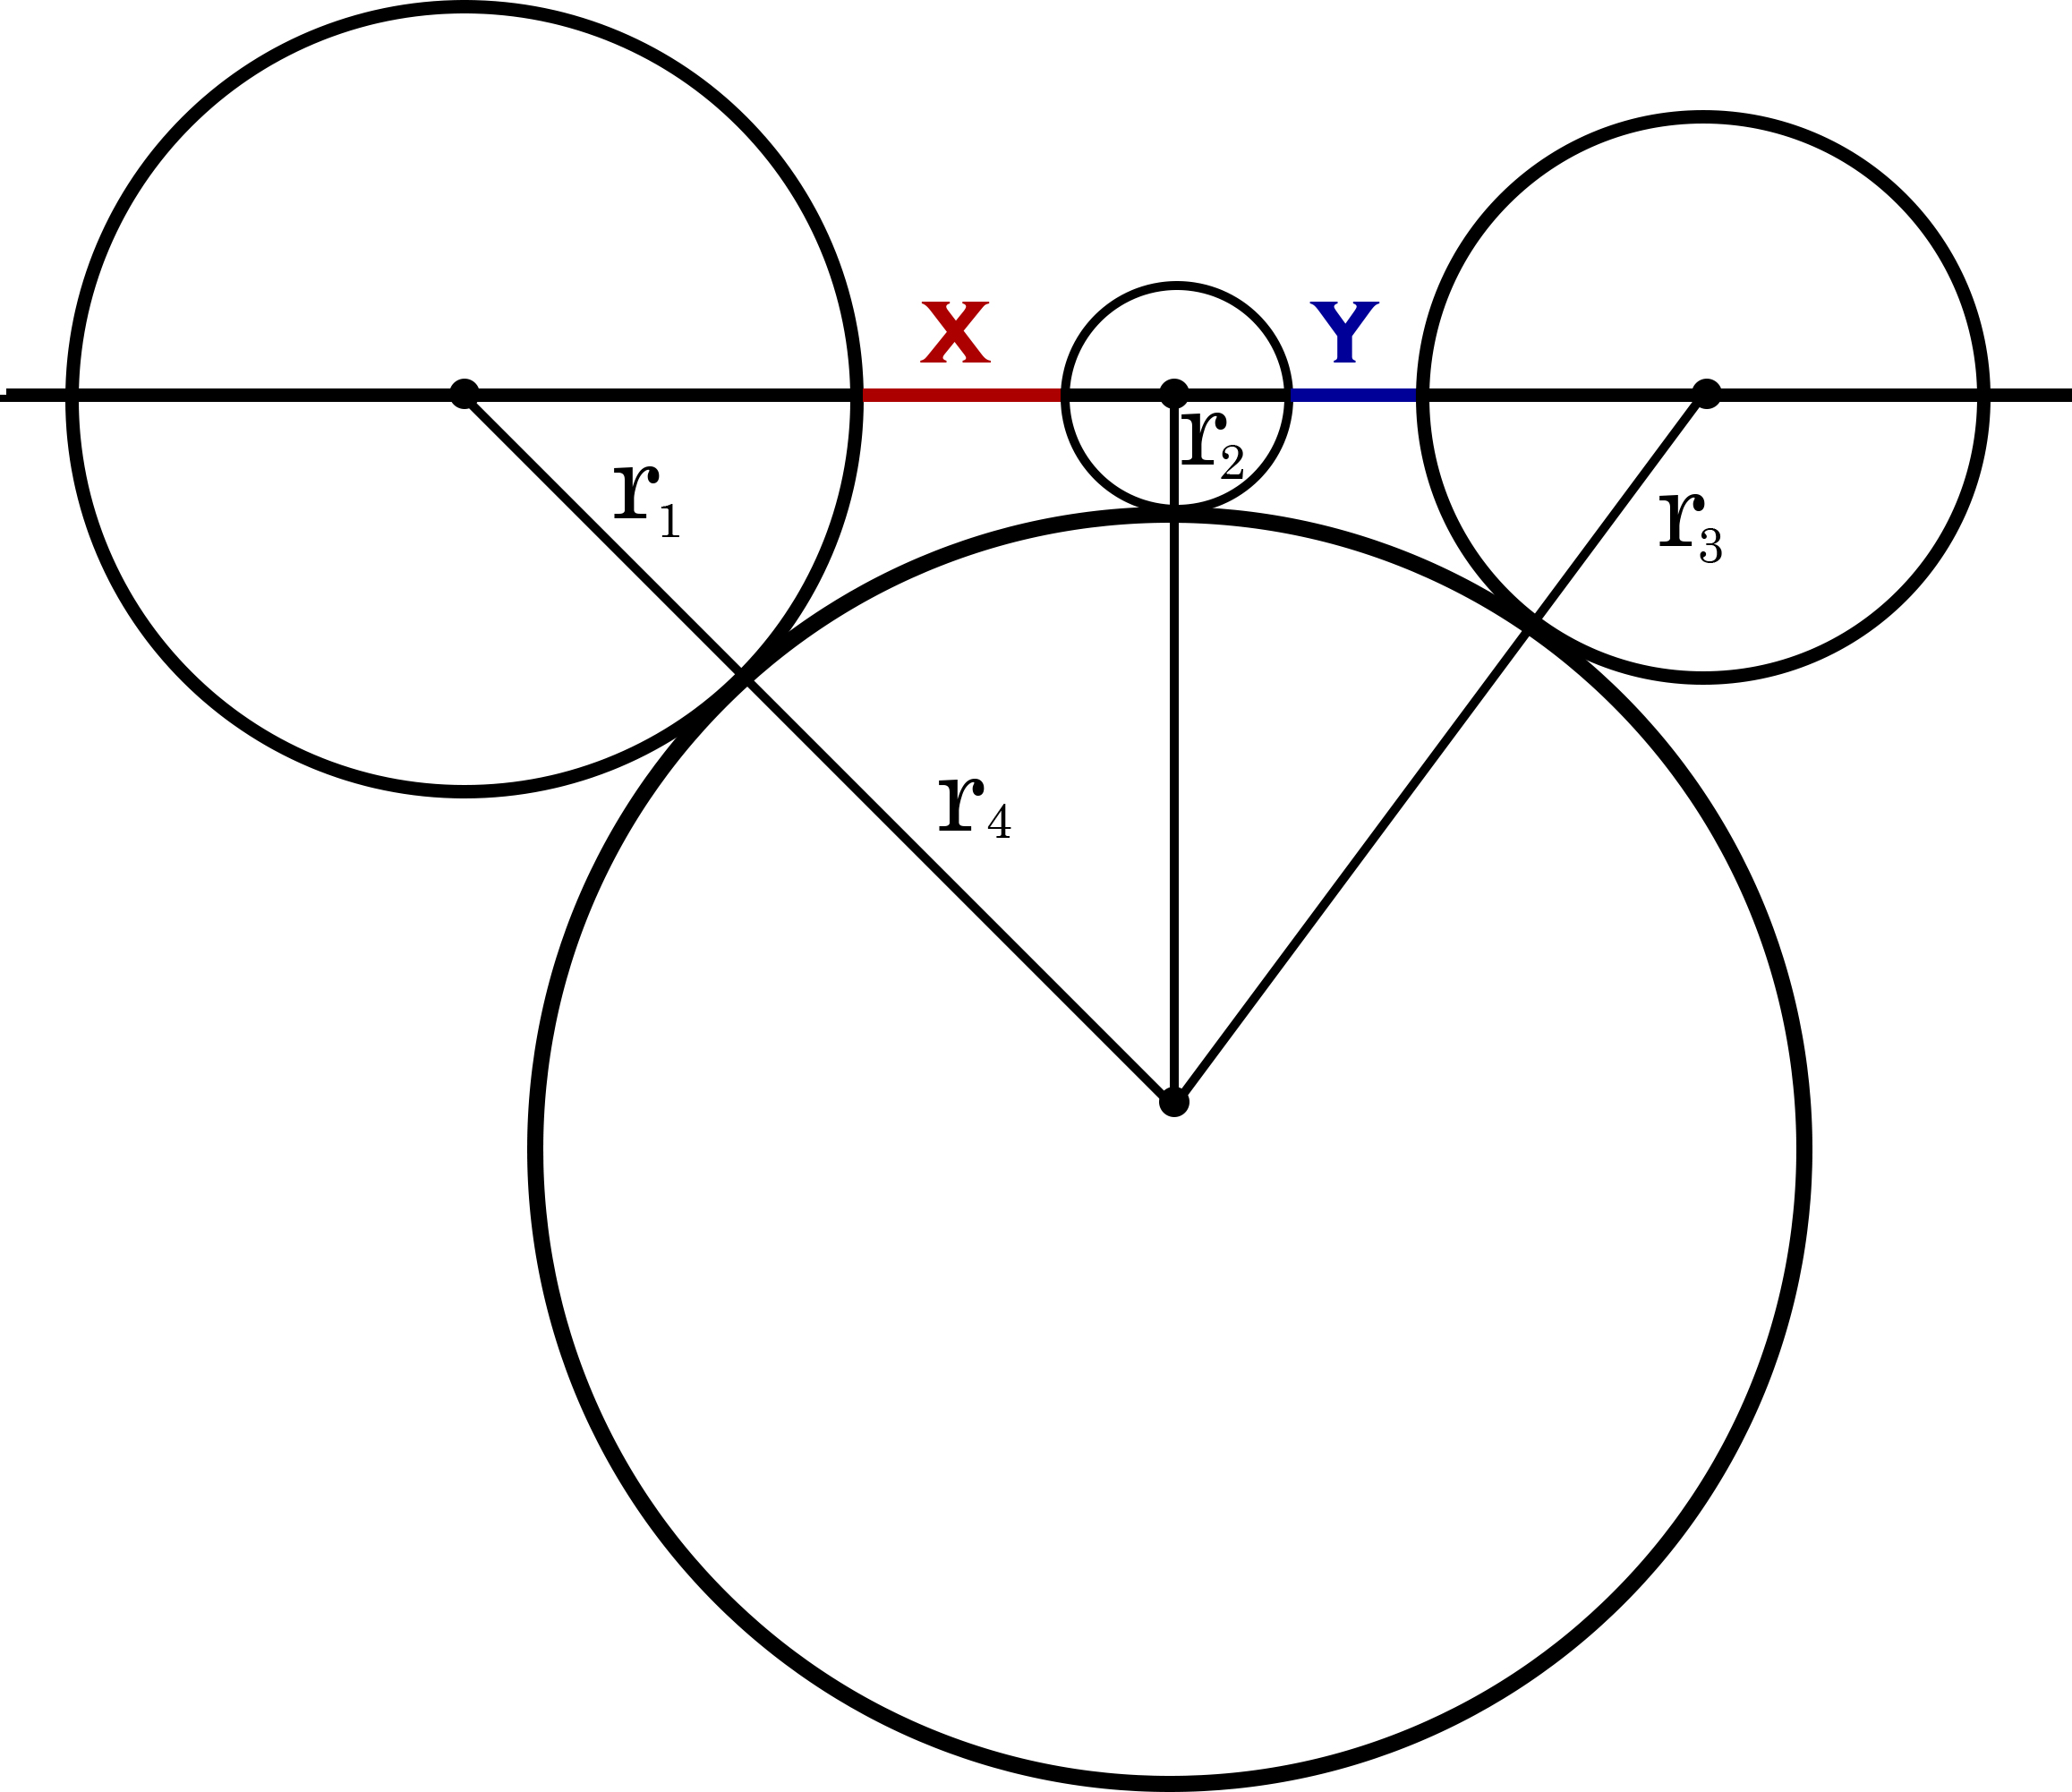
\includegraphics[width=0.6\textwidth]{\imgdirfromsection/exercicio-4circulos.jpg}
		\caption{Disposição dos quatro círculos.}
	\end{figure}
\end{exercise}

\begin{exercise}
Provar que em todo triângulo a soma dos comprimentos das
medianas é menor que o perímetro do triângulo e maior que o
semiperímetro (metade do perímetro) dele.
\end{exercise}

\begin{exercise}
  Suponha que $0 < a < b$. Prove que
$$a < \raiz{a \cdot b} < b.$$
\end{exercise}

\begin{exercise}
Prove que $a^4 +b^4 +c^4 \geq abc \prn{a+b+c}$.
\end{exercise}

\begin{exercise}
Sejam $a, b, c \in \R_+$. Prove que $$\prn {a+b} \prn {a+c}
\prn {b+c} \geq 8abc.$$
\end{exercise}

\begin{exercise}
  Sejam $a_1, a_2, ..., a_n \in \R^\ast_+$ tais que $a_1 \cdot a_2 \dots a_n = 1$. Mostre que $$\paren{1 + a_1 } \cdot \paren{1 + a_2} \dots \paren{1 + a_n } \geq 2^n.$$
\end{exercise}

\begin{exercise}
Sejam $a, b, c, d \in \R_+^*$. Prove que $$\prn {a+b+c+d}
\prn {\frac 1 a + \frac 1 b + \frac 1 c + \frac 1 d} \geq 16.$$
\end{exercise}


\begin{exercise}
A soma de três números positivos é 6. Prove que a soma de seus
quadrados não é menor que 12.
\end{exercise}
